\documentclass{article}
\usepackage{graphicx} % this package can be used for inserting graphics
\usepackage{amsmath} % this package includes the align environment
\usepackage{minted} % the minted package can be used to display code snippets
% with syntax highlighting in your documents.
\usepackage{float} % used to specify figure placement with high strictness
\begin{document}
\title{CS3505 Final Project, Fall 2020}
\author{Team Exoplanets\\Edward Barrowes, Corbin Gurnee, Ted Goodell,\\Marley Stark, Ivan Burkett, Garrett Keefe}
% The (build) date is included by default
\maketitle
\thispagestyle{empty} % removes the page number from this page
\newpage

\section{Overview}
  % Use prose to briefly describe your project and intended features
  \paragraph{}
  Our group project was to develop a web-scraping and data synthesizing tool that could use FFMPEG to create a scaled timeline of data from multiple sources. The project needed to be easily scaled, flexible, run remotely, and require minimal user input to generate timelines for arbitrary time windows. Additionally, we were tasked with making use of cloud storage to the best of our ability to support the architecture of our project.
  \paragraph{}
  We made use of multiple technologies in developing our tool, including:
  \begin{itemize}
    \item Amazon Web Services
    \item Docker
    \item GitHub
    \item Python
    \item Selenium
    \item FFMPEG
    \item C++
  \end{itemize}
  We were successful in meeting the aims of this project, including the educational aim of practicing AGILE development in a team based environment, all of which is outlined within this document.
\section{Architecture}
  \subsection{Organization}
  % Use prose and UML as appropriate to describe how your project parts are organized.
  \paragraph{}
  Scalability is an important goal for this project, which factors in to the organizational choices our team made. At the top level, all of our code is run on remote environments, and at lower levels is compartmentalized to allow for easy scalability.
  \paragraph{}
  The main operations of the program are run within a virtual machine instance using a service called Elastic Compute Cloud (EC2), which is itself a part of the greater Amazon Web Service (AWS). Within the EC2 instance are two Docker images: one for data collection, and one for data synthesis.
  \paragraph{}
  The data collection image uses a web-scraping tool called Selenium, to collect images and data from internet sources. Selenium supports multiple languages, but we chose to use python to interface with its scripts. These data are stored as .png images in cloud storage, again provided by Amazon, called the Elastic File System (EFS).
  \paragraph{}
  Data synthesis occurs within a Docker image containing code we constructed, framebuilder.cpp. framebuilder assembles individual images collected in the EFS, combining them into 600 time-consecutive frames using FFMPEG. Subsequently, the frames are assembled into a minute long video (again using FFMPEG) showing all of the data.
  \begin{figure}[H]
    \centering
    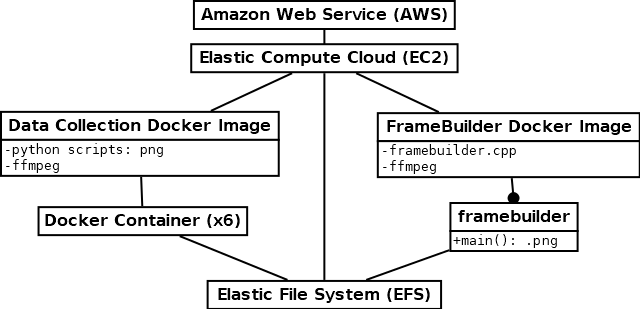
\includegraphics[width=0.8\linewidth]{img/class_diagram.png}
    \caption{UML Class diagram depicting project structure}
    \label{class_diagram}
  \end{figure}
  % notes to self
  % AWS runs a virtual machine (EC2), which runs continuously and runs docker images at regular time intervals using cron
  % EC2 runs docker containers using Dockerfiles we have made
  % 1 image has 6 containers which use python to collect data from their individual sources
  % Data is stored in the EFS (elastic file storage) in the form of images
  % At a time specified by the user, a video is built (framebuilder.cpp does this)
  %  framebuilder.cpp, which exists in the EFS, is run by the user.
  %   framebuilder.cpp calls ffmpeg code to make 600 frames, stored in EFS
  % The user runs an ffmpeg command to put the frames together, which outputs a video to whatever directory you want
  %   this happens in the same place that framebuilder exists (EFS)

  \subsection{Execution}
  % Use prose and UML as appropriate to describe how your project parts execute.
  \paragraph{}
  Execution occurs on both a continuous and instantaneous basis. Data collection occurs autonomously, and continuously, requiring no direct user input. Data synthesis occurs only when queried by the user interacting with the EC2 instance, illustrated below.
  \begin{figure}[H]
    \centering
    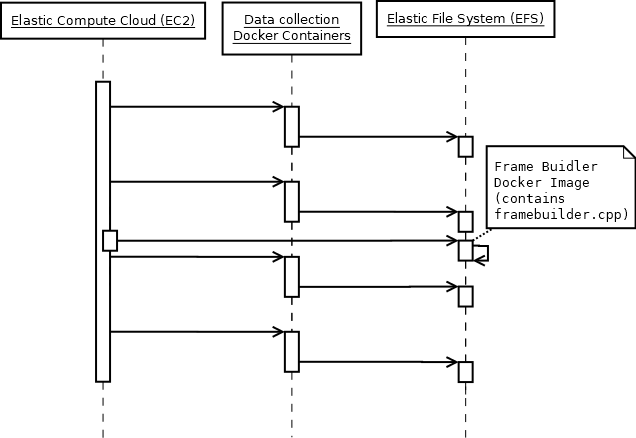
\includegraphics[width=0.8\linewidth]{img/sequence_diagram.png}
    \caption{UML Sequence diagram depicting project execution}
    \label{seuqence_diagram}
  \end{figure}
  \paragraph{}
  Autonomous data collection occurs at regular intervals, using the Linux command 'cron'. When data collection occurs, six Docker containers are instanced from the same image, each containing python code which collets data from various sources. The image itself contains all the code that all containers could need, however each data source updates at a different frequency. To compensate for this, we instance containers at appropriate time intervals in order to collect data.
  \paragraph{}
  A user can query the EC2 instance to produce a video compilation of collected data by running a bash script within the virtual machine. Running the script launches a Docker container, which contains our framebuilder.cpp program, which assembles all the data together into a minute long video. The container itself has FFMPEG installed, since framebuilder.cpp relies on its use.

\section{Development}
  \subsection{Organizational Tools}
  % Write a brief summary of the tools used to organize your project.
  To organize our project, we made use of GitHub and its associated functionality. All our code was backed by a git repository\footnote{https://github.com/xenonni/cs3505\_space\_data}, and our development progress was tracked using GitHub Projects and Issue Tracker.
  % Write/provide documentation from your planning software
  \begin{figure}[H]
    \centering
    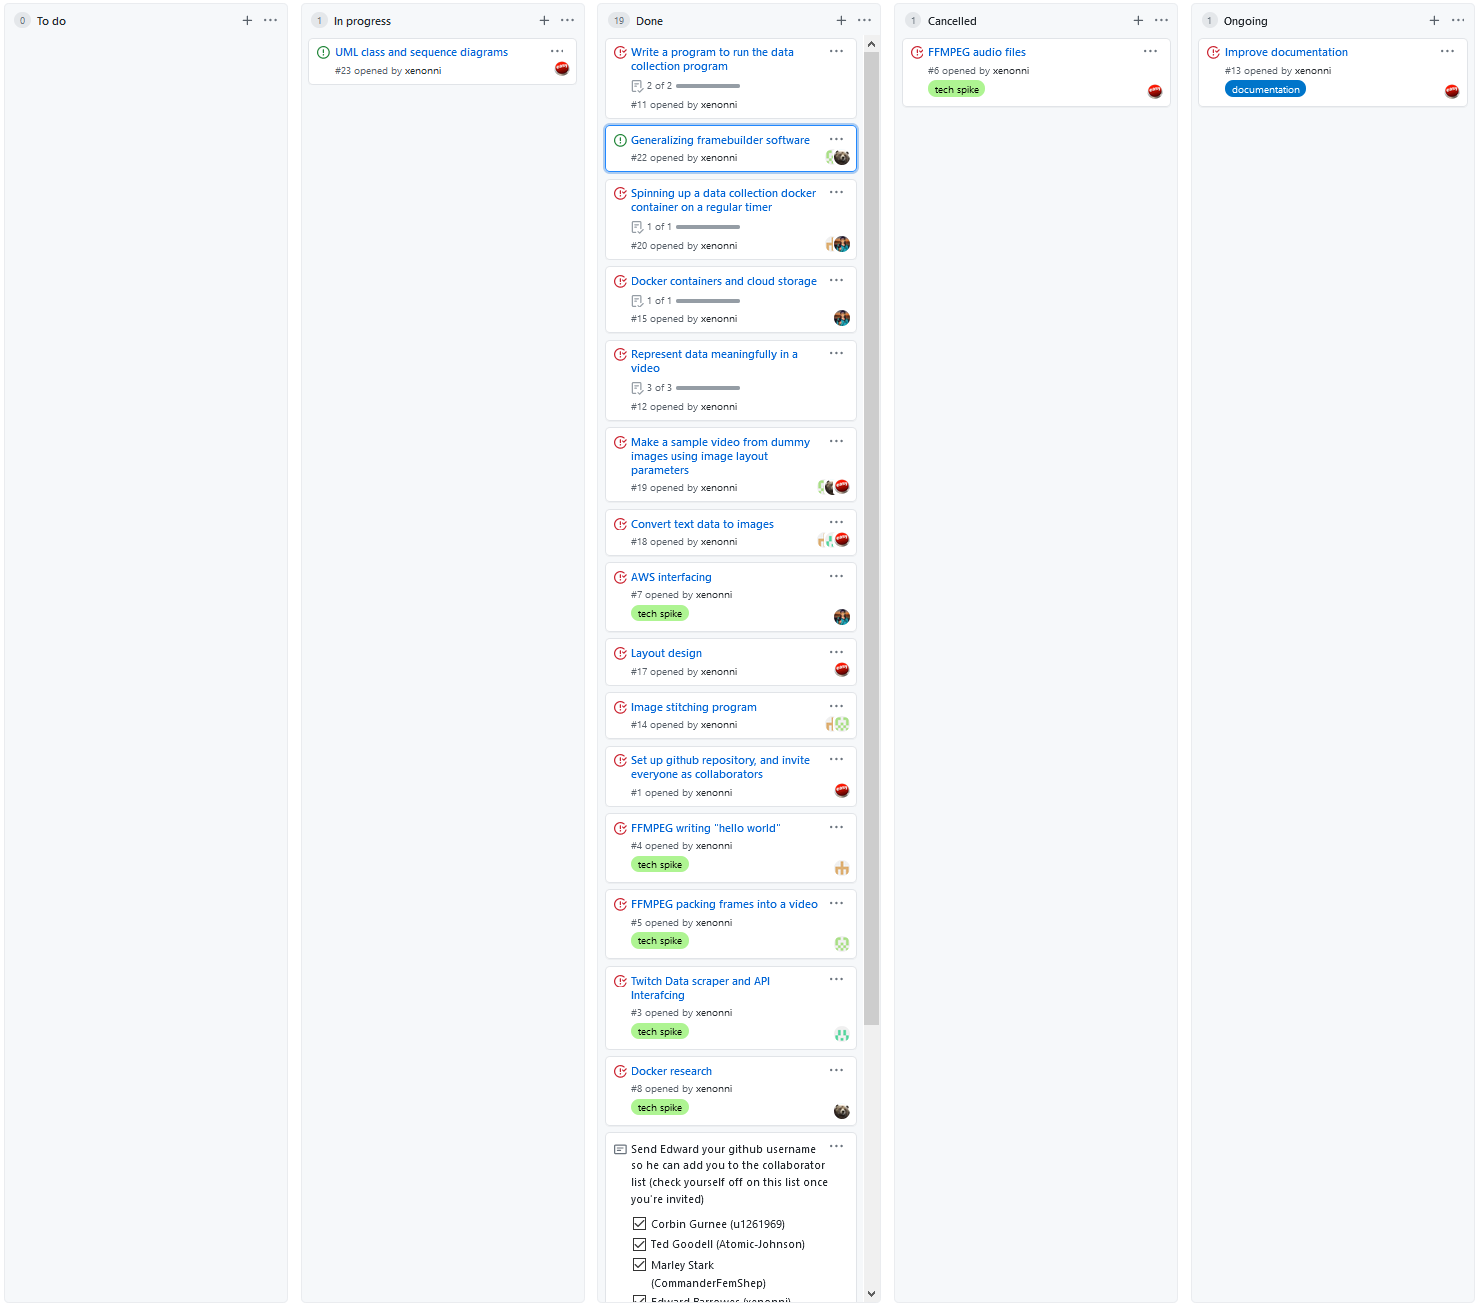
\includegraphics[width=0.75\linewidth]{img/github_projects.png}
    \caption{A screenshot showing the tracker, GitHub projects, which we used to organize development.}
    \label{github_projects}
  \end{figure}

  \begin{figure}[H]
    \centering
    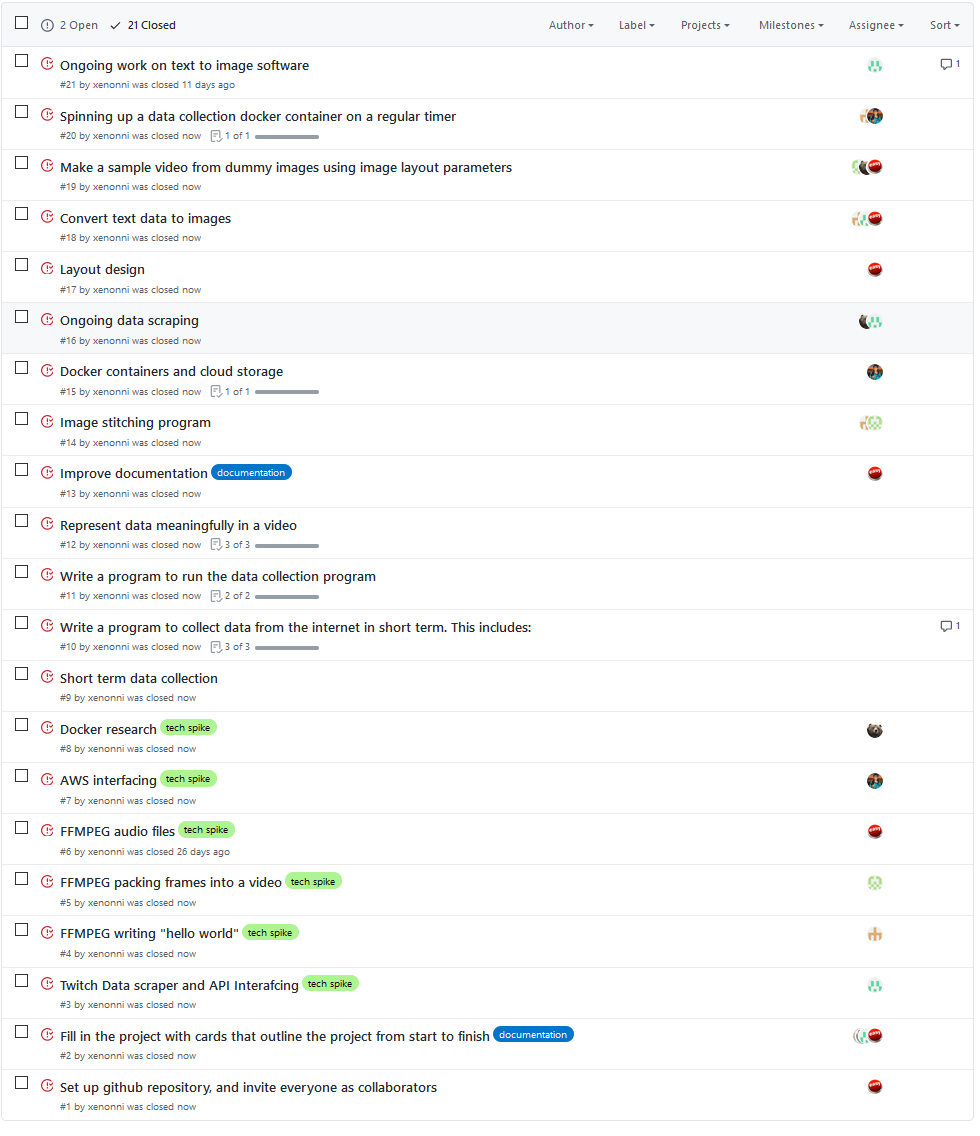
\includegraphics[width=\linewidth]{img/task_backlog.png}
    \caption{A screenshot showing a backlog of completed tasks (closed issues) in GitHub projects.}
    \label{backlog}
  \end{figure}
  Additionally, we took regular project development meeting notes, which were also stored in the repository and have been attached in appendix A.
  \newpage
  \subsection{Individual Reports}
    \paragraph{Corbin Gurnee -}
    For this project, I assisted with multiple parts. I was assigned to figure out how to work with API’s and how to get data with them. Thus I created a script to use the API on Twitch to gather the number of people watching the Science and Technology channel. After this I worked with Garret to create a Web scraper to get images off a webpage online. This turned out to be much easier than interacting with an API, so we changed all other scripts to run off of the web scraper as well. After this, I worked with Ted to convert the data we have compiled from our web scrapers to images. Finally, I worked in limited capacities with most other members of the team to assist in any area they may need assistance with.
    \paragraph{Ted Goodell -}
    I worked with Ivan on using the ffmpeg libraries to combine multiple images into a single image. To do this, we wrote code that decoded several images from their files and put them into frame structs that we could then programmatically combine into a larger frame. We then used the ffmpeg libraries to encode that frame and put it into an output image. I also, wrote python scripts that grabbed text data output by the data grabbers, and used the ffmpeg command line utility to put that text into an image. The ffmpeg command used a built in filter called “drawtext” to draw the text on a black template image for that portion of the final output image.
    \paragraph{Ivan Burkett -}
    I was assigned to work on the frame builder program for this project. I worked with Ted to create a C++ program called image-smoosh.cpp that used ffmpeg to combine the 6 frame segments into a single frame, then saved that frame as a png image. After finishing image-smoosh.cpp, I refactored the program to make it cleaner and easier to read and saved it as image-smoosh2.cpp. After doing that, I used image-smoosh2.cpp as a base to create framebuilder.cpp with Garrett. As part of making framebuilder.cpp, I also created a wrapper class for the C++ class directory-iterator called peek-directory-iterator, which simplified usage for directory-iterator and added a peek functionality which was necessary for our file traversal algorithm. framebuilder.cpp uses peek-directory-iterators to scan through the data source folders for the one most up to date for the provided date during the frame building process.
    \paragraph{Garrett Keefe -}
    I first worked on gathering research on docker and how it works. Then I was assigned with Corbin to work on the data scrappers to collect data from our 6 sources. I wrote all of the .py files which used selenium to navigate and grab web resources while Corbin wrote the twitch.out file which uses C++ and the curl libraries to query twitch.tv for info from its API. After that I was assigned to working with Ivan to create the framebuilder program which utilize UNIX timestamps to assemble data from our data sources and compile them together into individual frames, allowing us to generate a list of frames which we use an ffmpeg command to assemble them into a video. I also helped Ted create all of the .sh files which acted as drivers for our data collection and converting to picture formats within the docker containers.
    \paragraph{Edward Barrowes -}
    Most of my work on this project was in documentation and organization. I took meeting notes whenever we met and discussed anything of significance. Additionally, I was responsible for setting up the GitHub repository and populating the issue tracker with tasks we had discussed during meetings (though individual team members were responsible for updating progress on tasks they had been assigned). In addition to providing logistical support to the team, I also designed the final layout for the video based on the requirements and constraints the various data sources had. Lastly, as we finished the project, I was responsible for compiling our design discussions and sketches (from weekly meetings) into more professional communication, including this document and the UML diagrams contained within.
    \paragraph{Marley Stark -}
    I worked on AWS to get our EC2, EFS, and lambda functions set up so we could have a virtual environment on the cloud to automate and run our entire program and data collection. I made an AWS Educate account so we could explore what AWS provides without having to worry about being charged, and it seemed to have access to everything we needed for the assignment. However the AWS Educate account does not let you schedule EC2 instances so we were unable to set up the Cloudwatch events needed to use lambda functions on a schedule. Our lambda functions work to turn on and off our EC2, we just couldn’t schedule them to automate it. Taking advantage of Linux’s cron daemon, I edited the crontab file in Cloud9 to schedule our data collection jobs, and it works fantastic! So overall I navigated the immense world of AWS and made a Cloud9 EC2 instance and mounted an EFS to it, learned about Lambda functions and Cloudwatch but was unable to schedule things because of the AWS Educate account restrictions, and instead learned about and implemented cron jobs to do our automated data collection tasks.
\section{Results}
  % Write prose to describe the current project functionality
  According to the goals of our project, we have complete functionality. Our project works fully as intended because we can leave our EC2 instance running to collect data without having to even be signed into our AWS account. The timeline video is generated with minimal user input.
  \subsection{Running the Code}
  % Briefly indicate requirements and steps for running the project code.
   To make a video from the data you simply run the command “create\_video.sh mm.dd.yyyy.hh.ss mm.dd.yyyy.hh.ss” with the desired start and end times.
  % screenshot from the output video
  \begin{figure}[H]
    \centering
    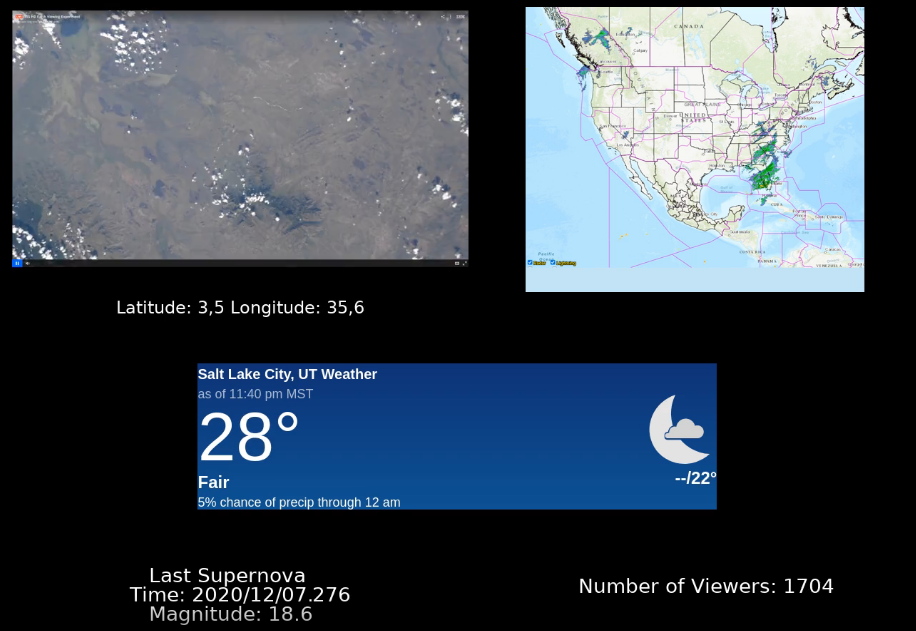
\includegraphics[width=\linewidth]{img/timeline_screenshot.png}
    \caption{A screenshot from the completed timeline.}
    \label{timeline}
  \end{figure}

\section{Appendix A: Meeting Notes}
%TODO Attach all the meeting notes as an appendix

\end{document}
